\subsection{ORDER RELATION AND OPERATIONS ON CARDINALS}

PROPOSITION 13. Let \(\mathfrak{a}\) and \(\mathfrak{b}\) be cardinals. Then \(\mathfrak{a} \geqslant \mathfrak{b}\) if and only if there exists a cardinal \(\mathfrak{c}\) such that \(\mathfrak{a} = \mathfrak{b} + \mathfrak{c}\) .

For the relation \(a \geqslant b\) means that there exists a subset B of a which is equipotent to b (no. 2), i.e., a is equipotent to the set which is the sum of b and a set c.

\pandocbounded{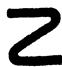
\includegraphics[keepaspectratio]{images/part002_f1d2aad8dae595af04a38c0526d2ebc1f30c28017ae785c1fe861e266dceeae2.jpg}}

If \(a \geqslant b\) , there usually exist many cardinals \(c\) such that \(a = b + c\) (cf.~§ 6); in general, therefore, it is not possible to define the ``difference'' \(a - b\) of two such cardinals (cf.~§ 5, no. 2).

PROPOSITION 14. Let \((\mathfrak{a}_i)_{i\in I}\) and \((\mathfrak{b}_i)_{i\in I}\) be two families of cardinals, both indexed by the same set \(I\) , and such that \(\mathfrak{a}_i\geqslant \mathfrak{b}_i\) for all \(i\in I\) . Then

\[
\sum_ {i \in I} a _ {i} \geqslant \sum_ {i \in I} b _ {i}, \quad \mathbf {P} _ {i \in I} a _ {i} \geqslant \mathbf {P} _ {i \in I} b _ {i}.
\]

The second inequality follows from the inclusion relations between products of sets (Chapter II, § 5, no. 4, Proposition 6, Corollary 3). As to the first inequality, if a set E is the union of a family \((\mathbf{A}_{t})_{t\in\mathbf{I}}\) of mutually disjoint subsets and if \(B_{t}\subset A_{t}\) for all \(t\in I\) , then the \(B_{t}\) are also mutually disjoint and \(\bigcup_{i}B_{i}\subset\bigcup_{i}A_{i}\) (Chapter II, § 4, no. 2).

COROLLARY 1. Let \((\mathfrak{a}_i)_{t \in I}\) be a family of cardinals. For each subset \(J\) of \(I\) we have \(\sum_{i \in J} \mathfrak{a}_i \leqslant \sum_{i \in I} \mathfrak{a}_i\) . If also \(\mathfrak{a}_i \neq 0\) for all \(i \in I - J\) , then \(\mathsf{P}_{i \in J} \mathfrak{a}_i \leqslant \mathsf{P}_{i \in I} \mathfrak{a}_i\) . Put \(\mathfrak{b}_i = \mathfrak{a}_i\) if \(i \in J\) , and \(\mathfrak{b}_i = 0\) (resp. \(\mathfrak{b}_i = 1\) ) if \(i \in I - J\) . Then apply Proposition 14, observing that the relation \(\mathfrak{a} \neq 0\) implies \(\mathfrak{a} \geqslant 1\) .

COROLLARY 2. If \(\mathfrak{a}\) , \(\mathfrak{a}'\) , \(\mathfrak{b}\) , \(\mathfrak{b}'\) are cardinals such that \(\mathfrak{a} \leqslant \mathfrak{a}'\) , \(\mathfrak{b} \leqslant \mathfrak{b}'\) , and \(\mathfrak{a}' > 0\) , then \(\mathfrak{a}^{\mathfrak{b}} \leqslant {\mathfrak{a}'}^{\mathfrak{b}'}\) .

For \(a^b \leqslant a'^b\) by Propositions 10 and 14, and \(a'^b \leqslant a'^{b'}\) by Proposition 10 and Corollary 1 to Proposition 14.

THEOREM 2 (Cantor). For each cardinal a, we have \(2^{\mathfrak{a}} > \mathfrak{a}\) .

We have \(\operatorname{Card}(\mathfrak{P}(\mathfrak{a})) = 2^{\mathfrak{a}}\) (no. 5, Proposition 12). The mapping \(x \to \{x\} (x \in \mathfrak{a})\) is an injection of \(\mathfrak{a}\) into \(\mathfrak{P}(\mathfrak{a})\) , whence \(\mathfrak{a} \leqslant 2^{\mathfrak{a}}\) . Hence it is enough to show that \(\mathfrak{a} \neq 2^{\mathfrak{a}}\) , i.e., that for every mapping \(f\) of \(\mathfrak{a}\) into \(\mathfrak{P}(\mathfrak{a})\) , the image \(f(\mathfrak{a})\) is distinct from \(\mathfrak{P}(\mathfrak{a})\) . Let \(\mathbf{X}\) be the set of all \(x \in \mathfrak{a}\) such that \(x \notin f(x)\) . If \(x \in \mathbf{X}\) , we have \(x \notin f(x)\) , whence \(f(x) \neq \mathbf{X}\) ; if \(x \in \mathfrak{a} - \mathbf{X}\) , we have \(x \in f(x)\) and \(x \notin \mathbf{X}\) , whence \(f(x) \neq \mathbf{X}\) . This shows that \(\mathbf{X} \notin f(\mathfrak{a})\) and proves the theorem.

COROLLARY. There does not exist a set that has every cardinal as an element.

If U were such a set, there would exist a set S, the sum of the family of sets \((\mathbf{X})_{\mathbf{x}\in\mathbf{U}}\) , so that every cardinal is equipotent to a subset of S. In particular, let \(\mathfrak{S}=\operatorname{Card}(\mathbf{S})\) ; since \(2^{S}\) is a cardinal, we would have \(2^{S}\leqslant S\) , in contradiction to Theorem 2.

